% Created 2025-01-14 mar 13:28
% Intended LaTeX compiler: pdflatex
\documentclass[10pt]{article}
\usepackage[utf8]{inputenc}
\usepackage{lmodern}
\usepackage[T1]{fontenc}
\usepackage[top=1in, bottom=1.in, left=1in, right=1in]{geometry}
\usepackage{graphicx}
\usepackage{longtable}
\usepackage{float}
\usepackage{wrapfig}
\usepackage{rotating}
\usepackage[normalem]{ulem}
\usepackage{amsmath}
\usepackage{textcomp}
\usepackage{marvosym}
\usepackage{wasysym}
\usepackage{amssymb}
\usepackage{amsmath}
\usepackage[theorems, skins]{tcolorbox}
\usepackage[version=3]{mhchem}
\usepackage[numbers,super,sort&compress]{natbib}
\usepackage{natmove}
\usepackage{url}
\usepackage[cache=false]{minted}
\usepackage[strings]{underscore}
\usepackage[linktocpage,pdfstartview=FitH,colorlinks,
linkcolor=blue,anchorcolor=blue,
citecolor=blue,filecolor=blue,menucolor=blue,urlcolor=blue]{hyperref}
\usepackage{attachfile}
\usepackage{setspace}
\usepackage[spanish]{babel}
\usepackage{fontspec}
\date{}
\title{Saldo de otros activos/pasivos con respecto al resto del mundo}
\begin{document}

\maketitle
\section*{Los datos}
\label{sec:orgfded846}

\begin{ABSTRACT}
Los datos de este ejercicio corresponden a la serie temporal de la
base de datos del \textbf{Banco de España} correspondiente la cuenta
financiera del \emph{saldo de otros activos/pasivos con respecto al resto
del mundo} (todos los sectores). Son datos trimestrales en miles de
euros.
\end{ABSTRACT}

\begin{quote}
Para abrir los datos debe estar instalada la base de datos del Banco
de España: ``Pinchar'' en menú desplegable: \emph{Archivo --> Bases de datos}
y pulsar en el icono \emph{Mirar en el Servidor}. Buscar en el listado la
base de datos \texttt{be} y pulsar con el ratón dos veces sobre ella.
\end{quote}


\begin{itemize}
\item Ficheros \url{https://github.com/mbujosab/EconometriaAplicada-SRC/tree/main/Ejercicios}
\begin{itemize}
\item Versión en \href{https://github.com/mbujosab/EconometriaAplicada-SRC/blob/main/SerieCuentasFinancierasBE.pdf}{pdf}
\item Datos: \url{SerieCuentasFinancierasBE.gdt}
\item Guión de gretl: \url{SerieCuentasFinancierasBE.inp}
\end{itemize}
\end{itemize}
\section*{Cuentas Financieras. Metodología SEC2010. Saldo. Otros activos/pasivos. Todos los sectores. Resto del mundo, Miles de Euros}
\label{sec:org08ae3d4}

\subsection*{Gráfico de la serie temporal y su correlograma:}
\label{sec:org8143e7c}

\begin{minted}[frame=lines,fontsize=\scriptsize,linenos=]{r}
gnuplot BE_2_5_8_16 --time-series --with-lines --output="otros.png"
corrgm BE_2_5_8_16 14 --plot="otrosACF-PACF.png"
\end{minted}

\begin{center}
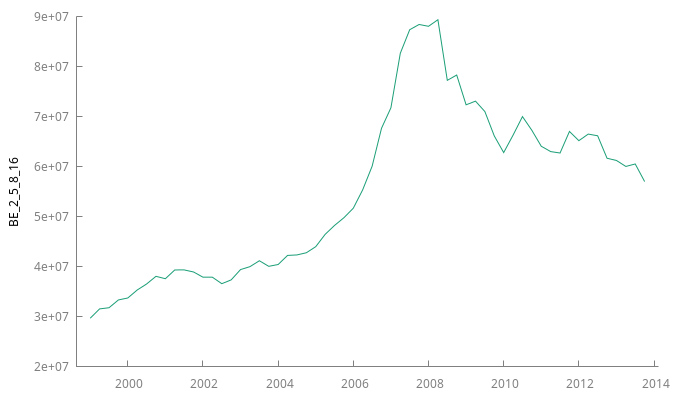
\includegraphics[width=0.5\textwidth]{./SerieCuentasFinancierasBE/otros.png} 
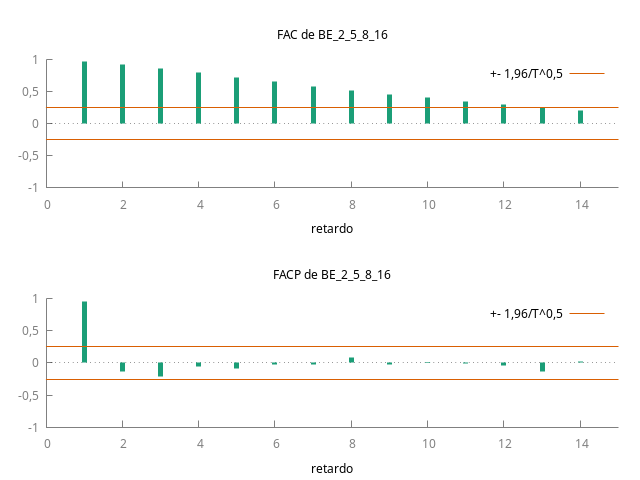
\includegraphics[width=0.4\textwidth]{./SerieCuentasFinancierasBE/otrosACF-PACF.png} 
\end{center}
\subsection*{Contrastes de raíz unitaria}
\label{sec:org5354606}
\subsubsection*{Contraste Dickey-Fuller aumentado de raíz unitaria}
\label{sec:org875f80d}

\begin{minted}[frame=lines,fontsize=\scriptsize,linenos=]{r}
adf 4 BE_2_5_8_16 --nc --test-down=AIC
\end{minted}

\begin{verbatim}
Contraste aumentado de Dickey-Fuller para BE_2_5_8_16
contrastar hacia abajo desde 4 retardos, con el criterio AIC
tamaño muestral 57
la hipótesis nula de raíz unitaria es: [a = 1]

  contraste sin constante 
  incluyendo 2 retardos de (1-L)BE_2_5_8_16
  modelo: (1-L)y = (a-1)*y(-1) + ... + e
  valor estimado de (a - 1): -0,000864383
  estadístico de contraste: tau_nc(1) = -0,122204
  valor p asintótico 0,6417
  Coef. de autocorrelación de primer orden de e: 0,005
  diferencias retardadas: F(2, 54) = 6,490 [0,0030]
\end{verbatim}
\subsubsection*{Contraste KPSS de estacionariedad}
\label{sec:org8a449ce}

\begin{minted}[frame=lines,fontsize=\scriptsize,linenos=]{r}
kpss 4 BE_1_2_1
\end{minted}

\begin{verbatim}
Contraste KPSS para BE_1_2_1

T = 60
Parámetro de truncamiento de los retardos = 4
Estadístico de contraste = 0,724905

                      10%      5%      1%
Valores críticos: 0,351   0,462   0,728
Valor p interpolado 0,010
\end{verbatim}
\section*{Datos en primeras diferencias}
\label{sec:org13cda42}

\begin{minted}[frame=lines,fontsize=\scriptsize,linenos=]{r}
diff BE_2_5_8_16
\end{minted}
\subsection*{Gráfico de la serie temporal en diferencias y su correlograma:}
\label{sec:orgd8e836a}

\begin{minted}[frame=lines,fontsize=\scriptsize,linenos=]{r}
gnuplot d_BE_2_5_8_16 --time-series --with-lines --output="d_otros.png"
corrgm d_BE_2_5_8_16 10 --plot="d_otrosACF-PACF.png"
\end{minted}

\begin{center}
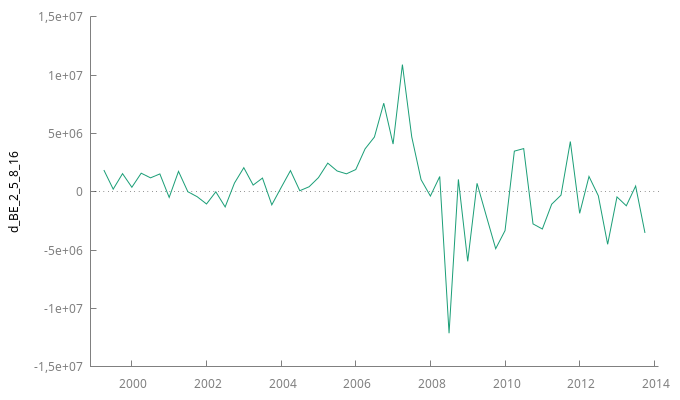
\includegraphics[width=0.5\textwidth]{./SerieCuentasFinancierasBE/d_otros.png} 
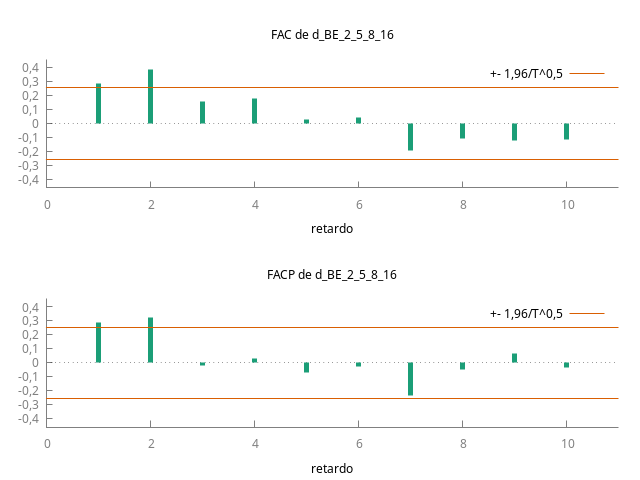
\includegraphics[width=0.4\textwidth]{./SerieCuentasFinancierasBE/d_otrosACF-PACF.png}
\end{center}
\subsection*{Contrastes de raíz unitaria}
\label{sec:org42feeeb}
\subsubsection*{Contraste Dickey-Fuller aumentado de raíz unitaria}
\label{sec:org6e44eec}

\begin{minted}[frame=lines,fontsize=\scriptsize,linenos=]{r}
adf 4 d_BE_2_5_8_16 --nc --test-down=AIC
\end{minted}

\begin{verbatim}
Contraste aumentado de Dickey-Fuller para d_BE_2_5_8_16
contrastar hacia abajo desde 4 retardos, con el criterio AIC
tamaño muestral 57
la hipótesis nula de raíz unitaria es: [a = 1]

  contraste sin constante 
  incluyendo un retardo de (1-L)d_BE_2_5_8_16
  modelo: (1-L)y = (a-1)*y(-1) + ... + e
  valor estimado de (a - 1): -0,455524
  estadístico de contraste: tau_nc(1) = -3,02904
  valor p asintótico 0,002394
  Coef. de autocorrelación de primer orden de e: 0,005
\end{verbatim}
\subsubsection*{Contraste KPSS de estacionariedad}
\label{sec:orgc812064}

\begin{minted}[frame=lines,fontsize=\scriptsize,linenos=]{r}
kpss 4 d_BE_2_5_8_16
\end{minted}

\begin{verbatim}
Contraste KPSS para d_BE_2_5_8_16

T = 59
Parámetro de truncamiento de los retardos = 4
Estadístico de contraste = 0,216133

                      10%      5%      1%
Valores críticos: 0,351   0,462   0,727
Valor p > .10
\end{verbatim}
\section*{Primer modelo univariante tentativo}
\label{sec:org5959734}


\begin{verbatim}
Evaluaciones de la función: 20
Evaluaciones del gradiente: 7

Modelo 2: ARIMA, usando las observaciones 1999:2-2013:4 (T = 59)
Estimado usando AS 197 (MV exacta)
Variable dependiente: (1-L) BE_2_5_8_16
Desviaciones típicas basadas en el Hessiano

              coeficiente    Desv. típica      z      valor p
  -----------------------------------------------------------
  const      416687          765151          0,5446   0,5860 
  phi_1           0,192168        0,122755   1,565    0,1175 
  phi_2           0,325667        0,122300   2,663    0,0077  ***

Media de la vble. dep.  463234,6   D.T. de la vble. dep.    3256442
Media de innovaciones  -15733,57   D.T. innovaciones        2915003
R-cuadrado              0,970881   R-cuadrado corregido    0,970370
Log-verosimilitud      -962,1093   Criterio de Akaike      1932,219
Criterio de Schwarz     1940,529   Crit. de Hannan-Quinn   1935,463

                       Real Imaginaria     Módulo Frecuencia
  -----------------------------------------------------------
  AR
   Raíz  1           1,4819     0,0000     1,4819     0,0000
   Raíz  2          -2,0720     0,0000     2,0720     0,5000
  -----------------------------------------------------------
\end{verbatim}
\subsection*{Residuos y su correlograma}
\label{sec:org536f78d}

\begin{minted}[frame=lines,fontsize=\scriptsize,linenos=]{r}
res1 = $uhat
gnuplot res1 --time-series --with-lines --output="res1.png"
corrgm res1 10 --plot="res1_ACF-PACF.png"
\end{minted}

\begin{center}
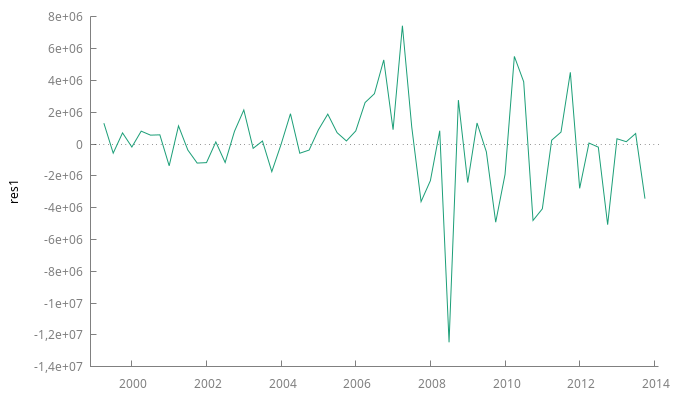
\includegraphics[width=0.5\textwidth]{./SerieCuentasFinancierasBE/res1.png} 
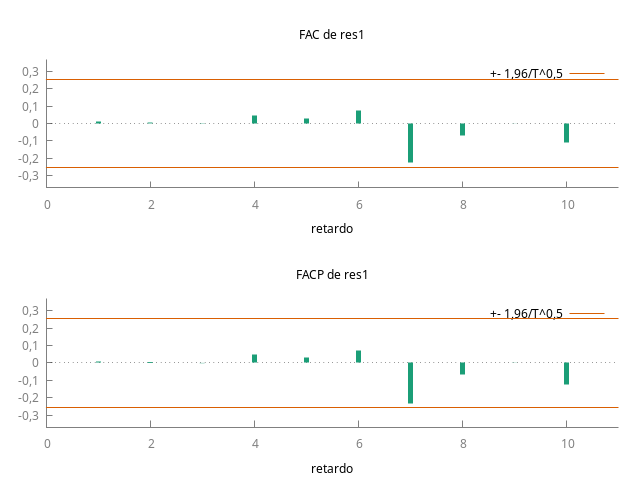
\includegraphics[width=0.4\textwidth]{./SerieCuentasFinancierasBE/res1_ACF-PACF.png}
\end{center}
\subsubsection*{Estadístico Ljung-Box para los residuos}
\label{sec:org5303992}

\begin{verbatim}
Función de autocorrelación para res1
***, ** y * indica significatividad a los niveles del 1%, 5% y 10%
utilizando la desviación típica 1/T^0,5

 RETARDO    FAC          FACP         Estad-Q. [valor p]

    1   0,0088        0,0088          0,0048  [0,945]
    2   0,0051        0,0051          0,0065  [0,997]
    3  -0,0017       -0,0018          0,0067  [1,000]
    4   0,0472        0,0473          0,1527  [0,997]
    5   0,0311        0,0304          0,2174  [0,999]
    6   0,0714        0,0707          0,5638  [0,997]
    7  -0,2278  *    -0,2308 *        4,1565  [0,762]
    8  -0,0685       -0,0691          4,4872  [0,811]
    9  -0,0007        0,0010          4,4872  [0,877]
   10  -0,1106       -0,1233          5,3855  [0,864]
\end{verbatim}
\section*{Segundo modelo univariante tentativo}
\label{sec:orgb6a76d6}

\begin{verbatim}
Evaluaciones de la función: 38
Evaluaciones del gradiente: 11

Modelo 4: ARIMA, usando las observaciones 1999:2-2013:4 (T = 59)
Estimado usando AS 197 (MV exacta)
Variable dependiente: (1-L) BE_2_5_8_16
Desviaciones típicas basadas en el Hessiano

              coeficiente    Desv. típica      z      valor p
  -----------------------------------------------------------
  const      436176          585387          0,7451   0,4562 
  theta_1         0,196262        0,122525   1,602    0,1092 
  theta_2         0,339626        0,125911   2,697    0,0070  ***

Media de la vble. dep.  463234,6   D.T. de la vble. dep.    3256442
Media de innovaciones  -7429,336   D.T. innovaciones        2955062
R-cuadrado              0,969732   R-cuadrado corregido    0,969201
Log-verosimilitud      -962,8936   Criterio de Akaike      1933,787
Criterio de Schwarz     1942,097   Crit. de Hannan-Quinn   1937,031

                       Real Imaginaria     Módulo Frecuencia
  -----------------------------------------------------------
  MA
   Raíz  1          -0,2889    -1,6914     1,7159    -0,2769
   Raíz  2          -0,2889     1,6914     1,7159     0,2769
  -----------------------------------------------------------
\end{verbatim}
\subsection*{Residuos y su correlograma}
\label{sec:org41c3e30}

\begin{minted}[frame=lines,fontsize=\scriptsize,linenos=]{r}
res2 = $uhat
gnuplot res2 --time-series --with-lines --output="res2.png"
corrgm res1 10 --plot="res2_ACF-PACF.png"
\end{minted}

\begin{center}
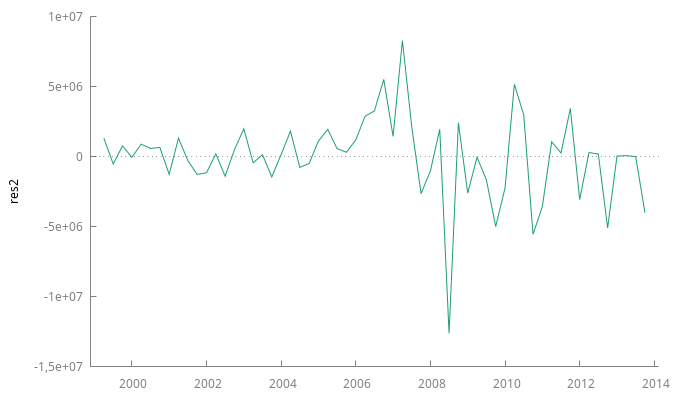
\includegraphics[width=0.5\textwidth]{./SerieCuentasFinancierasBE/res2.png} 
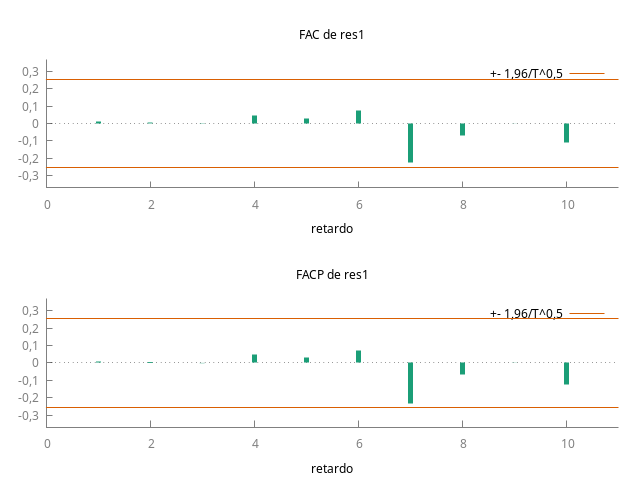
\includegraphics[width=0.4\textwidth]{./SerieCuentasFinancierasBE/res2_ACF-PACF.png}
\end{center}
\subsubsection*{Estadístico Ljung-Box para los residuos}
\label{sec:org1ef2009}

\begin{verbatim}
Función de autocorrelación para res2
***, ** y * indica significatividad a los niveles del 1%, 5% y 10%
utilizando la desviación típica 1/T^0,5

 RETARDO    FAC          FACP         Estad-Q. [valor p]

    1   0,0258        0,0258          0,0414  [0,839]
    2   0,0453        0,0447          0,1710  [0,918]
    3   0,1074        0,1054          0,9126  [0,822]
    4   0,1205        0,1153          1,8622  [0,761]
    5   0,0287        0,0165          1,9169  [0,861]
    6   0,0768        0,0572          2,3173  [0,888]
    7  -0,2228  *    -0,2579 **       5,7542  [0,569]
    8  -0,0422       -0,0653          5,8798  [0,661]
    9   0,0156        0,0144          5,8974  [0,750]
   10  -0,1513       -0,1226          7,5796  [0,670]
\end{verbatim}
\section*{Preguntas}
\label{sec:org609b09c}
\subsection*{Pregunta 1}
\label{sec:org493afb9}

Discuta de todas las formas posibles si la serie temporal
(\texttt{BE\_2\_5\_8\_16}) es estacionaria en media (i.e., si podemos asumir que
es una realización de un proceso estocástico estacionario en media),
usando para ello los resultados del apartado \hyperref[sec:org08ae3d4]{Cuentas Financieras. Metodología SEC2010. Saldo. Otros activos/pasivos. Todos los sectores. Resto del mundo, Miles de Euros} así como sus
subapartados.

(\hyperref[sec:org3ff719b]{Respuesta 1})
\subsection*{Pregunta 2}
\label{sec:orgcdf1092}

Discuta de todas las formas posibles si la primera diferencia de serie
temporal (\texttt{BE\_2\_5\_8\_16}) es estacionaria en media usando para ello los
resultados de los subapartados de la sección \hyperref[sec:org13cda42]{Datos en primeras diferencias}.

(\hyperref[sec:org4e26b41]{Respuesta 2})
\subsection*{Pregunta 3}
\label{sec:orga9286f5}

Destaque los principales resultados de cada uno de los dos modelos
univariantes.

(\hyperref[sec:orgbb1303e]{Respuesta 3})
\subsection*{Pregunta 4}
\label{sec:orgcb53583}

Compare los dos modelos univariantes. ¿Cuál considera que es mejor? ¿por qué?

(\hyperref[sec:org8637613]{Respuesta 4})
\subsection*{Pregunta 5}
\label{sec:org1e27c44}

¿Que modificaciones sugiere para el modelo que haya escogido en el
apartado anterior?

(\hyperref[sec:orge425bc0]{Respuesta 5})
\subsection*{Pregunta 6}
\label{sec:orgfa3ef62}

\begin{enumerate}
\item Escriba el primer modelo univariante en forma de ecuación ARIMA.
\item Escriba el segundo modelo univariante en forma de ecuación ARIMA.
\end{enumerate}

(\hyperref[sec:orge4ce92a]{Respuesta 6})
\section*{Respuestas}
\label{sec:org9b8c042}

\subsection*{Respuesta 1}
\label{sec:org3ff719b}

La serie \texttt{BE\_2\_5\_8\_16} parece ser NO estacionarias en media:
\begin{itemize}
\item En el gráfico se observa una persistente evolución creciente hasta
el año 2008 y decreciente tras 2008

\item La función de autocorrelación (FAC) muestra persistencia (sus
coeficientes decrecen despacio y a un ritmo aproximadamente lineal).
Además el primer coeficiente tiene un valor próximo a uno.

\item El contraste Dickey-Fuller aumentado no rechaza la hipótesis nula de
existencia de una raíz unitaria a niveles de significación
inferiores al 64\%.

\item En consonancia con lo anterior, el test KPSS rechaza que la serie
sea estacionaria tanto al 10\% como al 5\% (aunque por muy poco no lo
rechaza al 1\%).
\end{itemize}

\begin{quote}
\textbf{Aclaraciones a algunas respuestas incorrectas en los exámenes}:

\begin{itemize}
\item La identificación de un modelo ARIMA se hace analizando el
correlograma de datos de los que podamos asumir que son realización
de un proceso \emph{estacionario} (y el primer apartado precisamente
induce a rechazar que \texttt{BE\_2\_5\_8\_16} sea ``estacionaria'').

Por tanto, identificar un modelo a partir de los datos \texttt{BE\_2\_5\_8\_16}
en niveles \textbf{es completamente incorrecto} (pues no son estacionarios
y previamente hay que diferenciarlos). Consecuentemente, aunque el
primer retardo de la PACF es el único significativo (dado que la ACF
no decae exponencialmente) no podemos identificar que el modelo sea
un AR(1). Si quiere comprobarlo, estime un modelo AR(1) con los
datos en niveles, verá que los residuos no son (ni remotamente) la
realización de un proceso de ruido blanco; es decir, el modelo no es
un AR(1).
\end{itemize}


\begin{itemize}
\item Al realizar el contraste \textbf{KPSS} se rechaza (o quizá NO) la
\textbf{hipótesis nula del contraste KPSS}; es decir, la hipótesis \(H_0\):
\emph{el proceso es I(0)}. Por tanto, es incorrecto afirmar que al
realizar el contraste \textbf{KPSS} se rechaza la hipótesis nula del
contraste \textbf{ADF}, puesto que la \(H_0\) de este último contraste es que
\emph{el proceso es I(1)} (¡que es una hipótesis distinta!).
\end{itemize}


\begin{itemize}
\item Decir que ``se rechaza el \emph{contraste} ADF'' (o cualquier otro
\emph{contraste}) es incorrecto. Lo que se rechaza es la \emph{hipótesis nula}
del contraste (pero nunca el \emph{contraste}). Por poner otra analogía
absurda\(\ldots{}\) se mastica la comida que hay en el plato (pero no
se mastica ``el plato'').
\end{itemize}


\begin{itemize}
\item En el correlograma, el primer palote (tanto de la ACF como la PACF)
representa la magnitud de la autocorrelación de orden 1 (por tanto,
el ``palote'' NO ES UN AR(1)\(\ldots{}\) recuerde que un AR(1) es un
modelo y el palote representa el valor de un parámetro). Afirmar que
un AR (es decir un modelo autorregresivo) es muy próximo a uno no
tiene ningún sentido.

El primer primer ``palote'' de la ACF (y también de la PACF) es la
correlación de orden uno. Usted debe saber que la correlación es un
estadístico acotado entre -1 y 1, por tanto: JAMAS el primer
coeficiente de la PACF (o la ACF) será mayor que uno (o menor que
\(-1\)).
\end{itemize}
\end{quote}

(\hyperref[sec:org493afb9]{Pregunta 1})
\subsection*{Respuesta 2}
\label{sec:org4e26b41}

La serie \texttt{d\_BE\_2\_5\_8\_16} (la primera diferencia regular de
\texttt{BE\_2\_5\_8\_16}) parece ``estacionaria'' en media:
\begin{itemize}
\item Analizando el gráfico podemos observar que oscila de manera regular
alrededor de su media (aunque muestra un altibajo en su nivel en los
años 2007 y 2008, por lo que es importante analizar otros posibles
indicios que refuercen nuestra conclusión).

\item La función de autocorrelación (FAC) decae rápidamente (tan solo son
significativos los dos primeros retardos). El primer coeficiente
tiene un valor muy inferior a uno.

\item El contraste Dickey-Fuller aumentado rechaza contundentemente la
hipótesis nula de existencia de una raíz unitaria (\texttt{valor p
  asintótico 0,002394}).

\item En consonancia con lo anterior, el test KPSS NO rechaza que la serie
sea estacionaria ni siquiera al 10\% (por tanto tampoco al 5\% o al
1\%).
\end{itemize}

\begin{quote}
\textbf{Aclaraciones a algunas respuestas incorrectas en los exámenes}:

\begin{itemize}
\item No se rechazan los test de hipótesis, se rechazan las hipótesis
nulas de los contrastes (véase de nuevo las aclaraciones generales
al final del ejercicio \href{https://mbujosab.github.io/EconometriaAplicada-SRC/Ejercicios/LetrasTesoroAmericano3y6meses.html\#outline-container-org96e4dfc}{LetrasTesoroAmericano3y6meses}). Y es
\textbf{fundamental} indicar qué dice cada hipótesis en cada caso; decir
que se rechaza la hipótesis del contraste es no decir nada (véase de
nuevo las aclaraciones generales al final del ejercicio
\href{https://mbujosab.github.io/EconometriaAplicada-SRC/Ejercicios/LetrasTesoroAmericano3y6meses.html\#outline-container-org96e4dfc}{LetrasTesoroAmericano3y6meses}).
\end{itemize}



\begin{itemize}
\item El concepto de ``tendencia'' hace referencia a una descripción
(subjetiva) de la evolución a medio o largo plazo del \textbf{nivel} de la
serie. Por eso, en el caso de una serie ``estacionaria'', es mejor
decir: \emph{``en esta serie se aprecia un \textbf{nivel} aproximadamente
constante''}, en lugar de \emph{``una \textbf{tendencia} aproximadamente
constante''} (pues \emph{tendencia} hace referencia a la evolución del
nivel; y en una serie estacionaria se espera que el nivel se
mantenga estable, por eso, \emph{tendencia constante} es una expresión
poco adecuada).
\end{itemize}
\end{quote}


(\hyperref[sec:orgcdf1092]{Pregunta 2})
\subsection*{Respuesta 3}
\label{sec:orgbb1303e}

\begin{description}
\item[{Primer modelo.}] \textbf{Es un AR(2)} para la primera diferencia ordinaria
de la serie (\(\nabla \mathbf{y}\)); es decir, es un modelo
ARIMA(2,1,0). Las raíces del polinomio AR están claramente fuera del
círculo unidad (indicando que este modelo para la primera diferencia
de los datos es \textbf{estacionario}). Es más, mirando la ACF y la PACF se
aprecia que los residuos parecen ser una realización de un proceso
de ruido blanco, pues ningún retardo es estadísticamente
significativo y, sobre todo, los p-valores de los estadísticos de
Ljung-Box de los residuos son muy elevados, por lo que no se puede
rechazar la hipótesis nula de que los residuos sean ``ruido
blanco''. Por otra parte, aunque NI la constante NI el parámetro
correspondiente al primer retardo del modelo AR son estadísticamente
significativos, el modelo ajusta bastante bien los datos; pues tiene
un \(R^2\) muy elevado (\texttt{0,970881}).

\item[{Segundo modelo.}] \textbf{Es un MA(2)} para la primera diferencia
ordinaria de la serie (\(\nabla \mathbf{y}\)); es decir, es un modelo
ARIMA(0,1,2). Las raíces del polinomio MA están claramente fuera del
círculo unidad (indicando que este modelo para la primera diferencia
de los datos es \textbf{invertible}). Es más, al igual que en el modelo
anterior (y por los mismos motivos) no se puede rechazar la
hipótesis de que los residuos sean ``ruido blanco''. Por otra parte,
aunque NI la constante, NI el parámetro correspondiente al primer
retardo del modelo MA son estadísticamente significativos, este
modelo también ajusta muy bien los datos, pues tiene un \(R^2\) muy
elevado (\texttt{0,969732}).
\end{description}

\begin{quote}
\textbf{Aclaraciones a algunas respuestas incorrectas en los exámenes}:

\begin{itemize}
\item Lo primero y \textbf{fundamental} es indicar el tipo de modelo: si el
modelo es AR, MA o ARMA. Para ello es imprescindible indicar si es
un modelo de los datos en niveles o si lo es de los datos en
diferencias.

\item El \(R^2\) es el ratio entre la varianza de los datos ajustados y la
\textbf{varianza de los datos de la muestra} (en este caso de los datos de
la muestra \emph{en primeras diferencias}). Dado que la serie no es
estacionaria, hablar de la varianza del \emph{modelo} es
\textbf{incorrecto}. Como el modelo no es estacionario, pues incorpora una
diferencia ordinaria, la varianza no está definida. Consecuentemente
no tiene sentido hablar de \emph{la varianza del modelo} (aunque si lo
tiene hablar de la varianza de los datos).

Por otra parte, que el \(R^2\) esté próximo a 1 no significa que el
modelo sea muy \emph{``explicativo''}. Un modelo puede tener un \(R^2\) muy
elevado y simultáneamente ser completamente inútil para explicar
nada (hemos visto algunos ejemplos durante el curso\(\ldots{}\) repase
el tema sobre la correlación espuria).

Es habitual escuchar la coloquial expresión de que \emph{``un modelo
explica el \(X\) por ciento''} pero la frase no puede acabar ahí. Es
necesario completarla diciendo \emph{``el \(X\) por ciento de la varianza
de los datos''}.

Y no olvide que en realidad un \(R^2\) elevado, por sí solo, no
``explica'' nada.  El \(R^2\) en modelos con constante tan solo es un
ratio de varianzas. Y que solo cabe pretender dar una interpretación
a ese ratio si el modelo es \emph{previamente} considerado como una
descripción ``aceptable'' de la variable estudiada. Además, el verbo
\emph{``explica''} es un sinónimo ---mal escogido--- de \emph{``replica (o
reproduce)} un \(X\) por ciento de la varianza de los datos''.

\item Cuando se habla de si las raíces están fuera del círculo unidad,
\textbf{hay que especificar si las raíces son de un polinomio AR o MA},
pues la lectura es distinta en cada caso (``modelo estacionario'' en
el primer caso o ``modelo invertible'' en el segundo).

\item En un modelo \emph{univariante} no cabe hablar de correlaciones espurias
(eso corresponde a correlaciones entre dos series distintas)

\item Todo modelo AR es invertible (pues invertible significa que tiene
representación AR); consecuentemente decir AR ``invertible'' es como
decir: tengo un gato ``felino'' (¿hay alguno que no lo sea?).

\item Todo modelo MA es estacionario; consecuentemente decir MA
``estacionario'' es como lo del ``gato felino''.

\item El primer modelo univariante es un AR(2) y el segundo un
MA(2). Estos modelos son MUY DISTINTOS entre si. Afirmar que son
parecidos no está justificado de ningún modo. Lo que sí es parecido
entre ambos es \emph{el nivel de ajuste} logrado por cada uno de ellos.

\item Un retardo significativo en la ACF o la PACF no es ``un
atípico''. Aunque algunos datos pueden ser calificados de atípicos,
los retardos de un correlograma NO.

\item La alusión a los \(R^2\) \emph{ajustados} o los \emph{criterios de información}
no debe hacerse aquí. Debe hacerse en la \hyperref[sec:orgcb53583]{Pregunta 4}, que es donde se
pide comparar los dos modelos de la misma variable \texttt{d\_BE\_2\_5\_8\_16}

\item Afirmar (y transcribo literalmente): \emph{``El módulo del AR resulta ser
mayor que uno''} NO TIENE SENTIDO. En todo caso sería \textbf{el módulo de
la raíz del polinomio AR}. Pero en este caso hay dos raíces, por lo
que la frase tiene aún menos sentido. Lo que se puede decir del
primer modelo es que las dos raíces del polinomio autorregresivo
tiene módulos mayores que uno (o que ambas raíces autorregresivas
están fuera del círculo unidad).

Peor aún (y vuelvo a transcribir): \emph{``MA \textbf{contiene} un modulo mayor
que uno''} (la negrita es mía pero la frase es del mismo examen).

En algún otro examen he leído: \emph{el modelo univariante no presenta MA
y solo AR}\ldots{} otra frase más de esas sin ningún sentido\ldots{}

\textbf{En un examen escrito se debe cuidar especialmente el lenguaje, para
lograr construir expresiones con pleno significado. Para ello se
debe escoger correctamente el vocabulario; y esto solo es posible
tras una adecuada comprensión de los conceptos}.
\end{itemize}
\end{quote}


(\hyperref[sec:orga9286f5]{Pregunta 3})
\subsection*{Respuesta 4}
\label{sec:org8637613}

Respecto a la identificación de los modelos: el correlograma de la
serie en diferencias muestra un decaimiento más lento en la ACF que en
la PACF; de hecho, la PACF muestra un abrupto decaimiento en el tercer
retardo. \textbf{Esto sugiere que el modelo es un AR(2)}.

En cuanto al \(R^2\) \emph{ajustado}, es ligeramente superior en el primer
modelo (en consonancia con ello la desviación típica de las
innovaciones del primer modelo es menor). Además, los criterios de
información son ligeramente inferiores en el primer modelo. Todos
estos estadísticos apuntan a una ligera ventaja del primer modelo
frente al segundo. Es más, los estadísticos de Ljung-Box para los
residuos del primer modelo muestran unos p-valores sistemáticamente
superiores a los del segundo. 

Todo lo anterior, \uline{indica que el primer modelo es más adecuado que el
segundo.}

\begin{quote}
\textbf{Aclaraciones a algunas respuestas incorrectas en los exámenes}:

\begin{itemize}
\item El \emph{p}-valor es una probabilidad: la probabilidad (bajo la \(H_0\)) de
que una variable aleatoria con la misma distribución del estadístico
del contraste, tome un valor ``más extremo'' que el observado en la
muestra (con más extremo queremos decir, más en el ``interior'' de
la región crítica).

\item Consecuentemente, hablar del \emph{p}-valor de los residuos no tiene
sentido. Lo que si tiene sentido es referirse a los \emph{p}-valores de
los estadísticos del contraste Ljung-Box realizado sobre los
residuos.
\end{itemize}
\end{quote}


(\hyperref[sec:orgcb53583]{Pregunta 4})
\subsection*{Respuesta 5}
\label{sec:orge425bc0}

Ambos modelos tienen parámetros no significativos. Por tanto cabe la
posibilidad de que el modelo mejore si se restringe la estimación para
que tanto la constante como el parámetro correspondiente al primer
retardo (en los respectivos modelos) sean cero. Es decir, cabe la
posibilidad de que el modelo mejore si se eliminan los parámetros no
significativos del modelo.

\begin{quote}
\textbf{Aclaraciones a algunas respuestas incorrectas en los exámenes}:

\begin{itemize}
\item Un modelo en el que \(\phi_1=0\) pero \(\phi_2\ne0\) sigue siendo un
modelo AR(2); del mismo modo \(1-x+x^2\) es un polinomio de grado 2,
pero también lo es \(1+x^2\) o incluso \(7x^2\). El orden del modelo AR
lo da el mayor \emph{retardo} significativo (y no el número de parámetros
significativos).

\item Lo mismo se puede decir de los modelos MA.
\end{itemize}
\end{quote}



(\hyperref[sec:org1e27c44]{Pregunta 5})
\subsection*{Respuesta 6}
\label{sec:orge4ce92a}

Redondeando:
\begin{description}
\item[{El primer modelo es:}] \(\quad(1-0,192\ \mathsf{B}-0,326\ \mathsf{B}^2)\nabla Y_t = 416687 +U_t\)

\item[{El segundo modelo es:}] \(\quad\nabla Y_t = 436176 + (1+0,196\ \mathsf{B}+0,340\ \mathsf{B}^2) U_t\)
\end{description}

(\hyperref[sec:orgfa3ef62]{Pregunta 6})
\end{document}
